\section{Introduction}

% Situation
Today geospatial web services are widely deployed on the web. A significant subset of these services can be queried using bounding box requests to retrieve geospatial data, either in raster or vector form, within a region. The classic example of such a service is Web Map Service (WMS). In WMS, results are typically computed on-the-fly by pulling data from a geospatial database. This strategy has the advantage that results are always up-to-date and it thus offers a great degree of flexibility and accuracy to clients of the service. At a high level, we can think of the service as applying a \emph{rendering function} to a set of matched base data to produce, e.g., a map image.

% Problem
Services that apply rendering functions in response to bounding box requests are often CPU- and I/O-intensive, with relatively high latency as a consequence. This is a problem because geospatial services are typically used interactively, and latency in excess of a few hundreds of milliseconds becomes noticeable. Even if the computation is not that expensive, the infrastructure available might not scale to many simultaneous users, if data is to be computed on demand. We know from our studies of government production services that may use as much as 30 seconds to compute a 256 x 256 pixel map image, which severely lowers the value of the service in an interactive scenario. On the other side, limiting the use of GIS to working with results that can be computed fast, does not generally seem like a good idea. While the issue of high latency can to a certain degree be dealt with by scaling up or out, such solutions do not come without a cost, e.g. increased power consumption and hardware costs. Instead of simply adding more resources, better algorithms can be developed to deal with high latency.

% State of the art
Real-world workloads contain significant amounts of repeated requests and often a strong skew in what is requested~\cite{fisher07,talagala00}. This offers an opportunity to replay the results of previous computations by placing geospatial results in a cache. A common approach to representing a set of geospatial results at multiple resolutions is to use a tiling scheme that divides a geographical data set into a hierarchical and finite set of \emph{tiles}~\cite{decola93}. Unfortunately, the drawback of this approach is that the set of tiles is potentially very large~\cite{garcia11}, as the number of tiles is exponential in the number of supported resolutions. It is common to fix the number of resolutions when dealing with tiles, and thus we assume a fixed set of resolutions. Even then, the sheer number of tiles makes computing and storing all of them difficult to manage.

Two primary approaches have been suggested for dealing with the delivery of tiles to clients: \emph{online} and \emph{off-line}. The online approach attempts to mask the latency of computing tiles on-demand for a single user, by prefetching tiles based on predictions of future accesses given the user's current viewstate~\cite{KKK01:Prefetching,KKK01:Prefetching2,LKK+02:Prefetching}. The off-line approach is to materialize a large but polynomial number of tiles in advance that is expected to cover to the majority of user request in the near future. It is assumed that serving the materialized tiles from a cache will be less CPU- and I/O-intensive than computing them on demand. The main problem then becomes selecting a good set of tiles. 

A drawback to the online approach is that although pre-fetching theoretically masks latency for a single user, it does not by itself decrease global concurrency, as tiles are still computed on demand. We speculate that this approach could even increase the average latency if view states are mispredicted. A drawback with materializing a set of tiles offline is that the tiles might not be up-to-date by the time they are requested, but this can be solved by invalidating the stale tiles. We will focus on the latter off-line approach in our work.

The off-line approach takes a global view of the problem, and aims at predicting a ``good'' set of tiles, i.e., a set containing tiles that are likely to be requested by many users in the near future. We argue that these tiles should be materialized during a window of low load. This strategy avoids impacting latency negatively in the high load period, but holds the potential to reduce average latency because of pre-computation.

% which in turn increases the average global latency, in order to decrease the latency for a particular user. 
Methods in the literature use rule-based algorithms to select which tiles should be materialized ahead of time~\cite{quinn10}. The rules are based on \emph{a priori} knowledge of user behavior, so a drawback of these methods is that the rules do not adapt to changes in user behavior over time. In addition, rule-based methods are hard to adapt to shorter time windows of low load. As they offer only limited insight over which tiles are the most relevant among the tiles selected by the rules, it is hard to choose a good subset of tiles to be materialized under a time constraint.  
% MVS: are there other rule-based approaches that we can cite? Does anybody cite Quinn and Gahegan?

In this paper, we present an adaptive tile selection method, \emph{TileHeat}, which suffers significantly less from these drawbacks. TileHeat is based on  \emph{a posteriori} knowledge of user behavior gathered from historical usage of the geospatial web service. We investigate algorithms that predict the set of tiles that will be requested in time period $t + 1$, and that are trained using a log of requests for periods $t-n, t -n + 1, \ldots, t$. Our algorithms construct a set of $n$ spatial heatmaps of requests, one for each time period, and uses these to predict future requests. To avoid over-fitting the model to the training data, we use both exponential smoothing and heat dissipation on the constructed heatmaps. The output of our algorithms is a ranking of tiles based on predicted likelihood of access for the next time period. As such, the number of tiles to be pre-computed can be chosen according to the available time window of low load.	

\minisec{Outline and Contributions}
Our paper starts with a discussion of existing methodologies for tile caching (Section~\ref{sec:tile:caching}). Then the main \emph{contributions} of the paper follow:
%
\begin{itemize}

\item We analyze a sample from the production log of The Digital Map Supply, a production geospatial web service maintained by the National Survey and Cadastre (KMS) in Denmark. In Section~\ref{sec:analysis}, we present our key observations of the workload, e.g. that the load curve follows a pattern with high load in the middle of the day, and low load in the rest of the day, and that the spatial distribution of requests is very stable over time.

\item We present the general framework of TileHeat, and propose a set of algorithms for ranking tiles. The algorithms exploit the properties we have discovered in the analysis, namely by tracking and predicting the spatial distribution of requests using heatmaps (Section~\ref{sec:algorithms}).

\item We present an experimental evaluation of the effectiveness of TileHeat. We observe an improvement of $25\%$ over the existing method used in the production system of KMS  for a set of tiles that can be materialized during an observed time window of low load (Section~\ref{sec:experiments}).

\end{itemize}
%
We end the paper by reviewing additional related work (Section~\ref{sec:related}). 


\section{Background}
\label{sec:tile:caching}

A \emph{tile cache} is a widely used method for dealing with the bad performance of services that render results from base data on-the-fly, such as WMS and similar services. In the following, we discuss the main concepts (Sections~\ref{sec:tile:pyramid} to~\ref{sec:heatmap:model}) and existing methods (Section~\ref{sec:existing:methods}) in tile caching.

\subsection{The Tile Pyramid}
\label{sec:tile:pyramid}

Tile caches are based on a model called a \emph{tile pyramid}, which subdivides a geographical region into a finite number of subregions using a set of $l$ grids~\cite{decola93}. In Figure~\ref{fig:tilepyramid}, a tile pyramid with three levels is shown. The cells of the grids are called \emph{tiles}, and tiles are indexed by a triple $(i,j,z)$. In this triple $z$ identifies a grid, while $i$ and $j$ represent the row and column in the grid where the tile is located. Each grid is associated with a data set at a particular resolution in meters per pixel. Tiles thus correspond to data at a given resolution, and within a bounding box.

\begin{figure}
\centering

\includegraphics[scale=0.8]{figs-tileheat/tilepyramid}
\caption{Tile pyramid with three levels $z=\{1, 2, 3\}$ shown. Level $z=1$ has dimensions $(1,1)$. Figure is reproduced from \cite{quinn10}}
\label{fig:tilepyramid}
\end{figure}

When a tile cache is initialized, all tiles point to $null$. A tile is materialized by making it point to geographical data stored on disk. The geographical data is rendered from a set of base objects, and if the base objects are updated the tile becomes \emph{stale}. Stale tiles are removed to avoid serving stale data to clients.

One shortcoming of tile caches is that the number of tiles is exponential in $l$, with grid $i+1$ containing four times as many tiles as grid $i$. This means that a tile cache consumes $O(4^l)$ in storage, and $O(4^l)$ time is required to materialize all tiles. A pyramid of $l=20$ levels requires several petabytes of storage \cite{garcia11}. The throughput of computing tiles has been reported by KMS to be around $58$ tiles per second on their infrastructure \cite{lindegaard12}. At this rate of computing tiles, it would take approximately $200$ years to compute the $3.7 \times 10^{11}$ tiles needed~\cite{garcia11}.

\subsection{Processing user requests}
\label{sec:processing:user:requests}
We abstract user requests to a geospatial web service by two functions: \texttt{GET} and \texttt{PUT}. \texttt{GET} retrieves a tile from a web service, while \texttt{PUT} updates the base data from which tiles are computed. Pseudocode for processing \texttt{GET} and \texttt{PUT} requests are given in Figure \ref{fig:pseudocode}.

\begin{figure}[h]
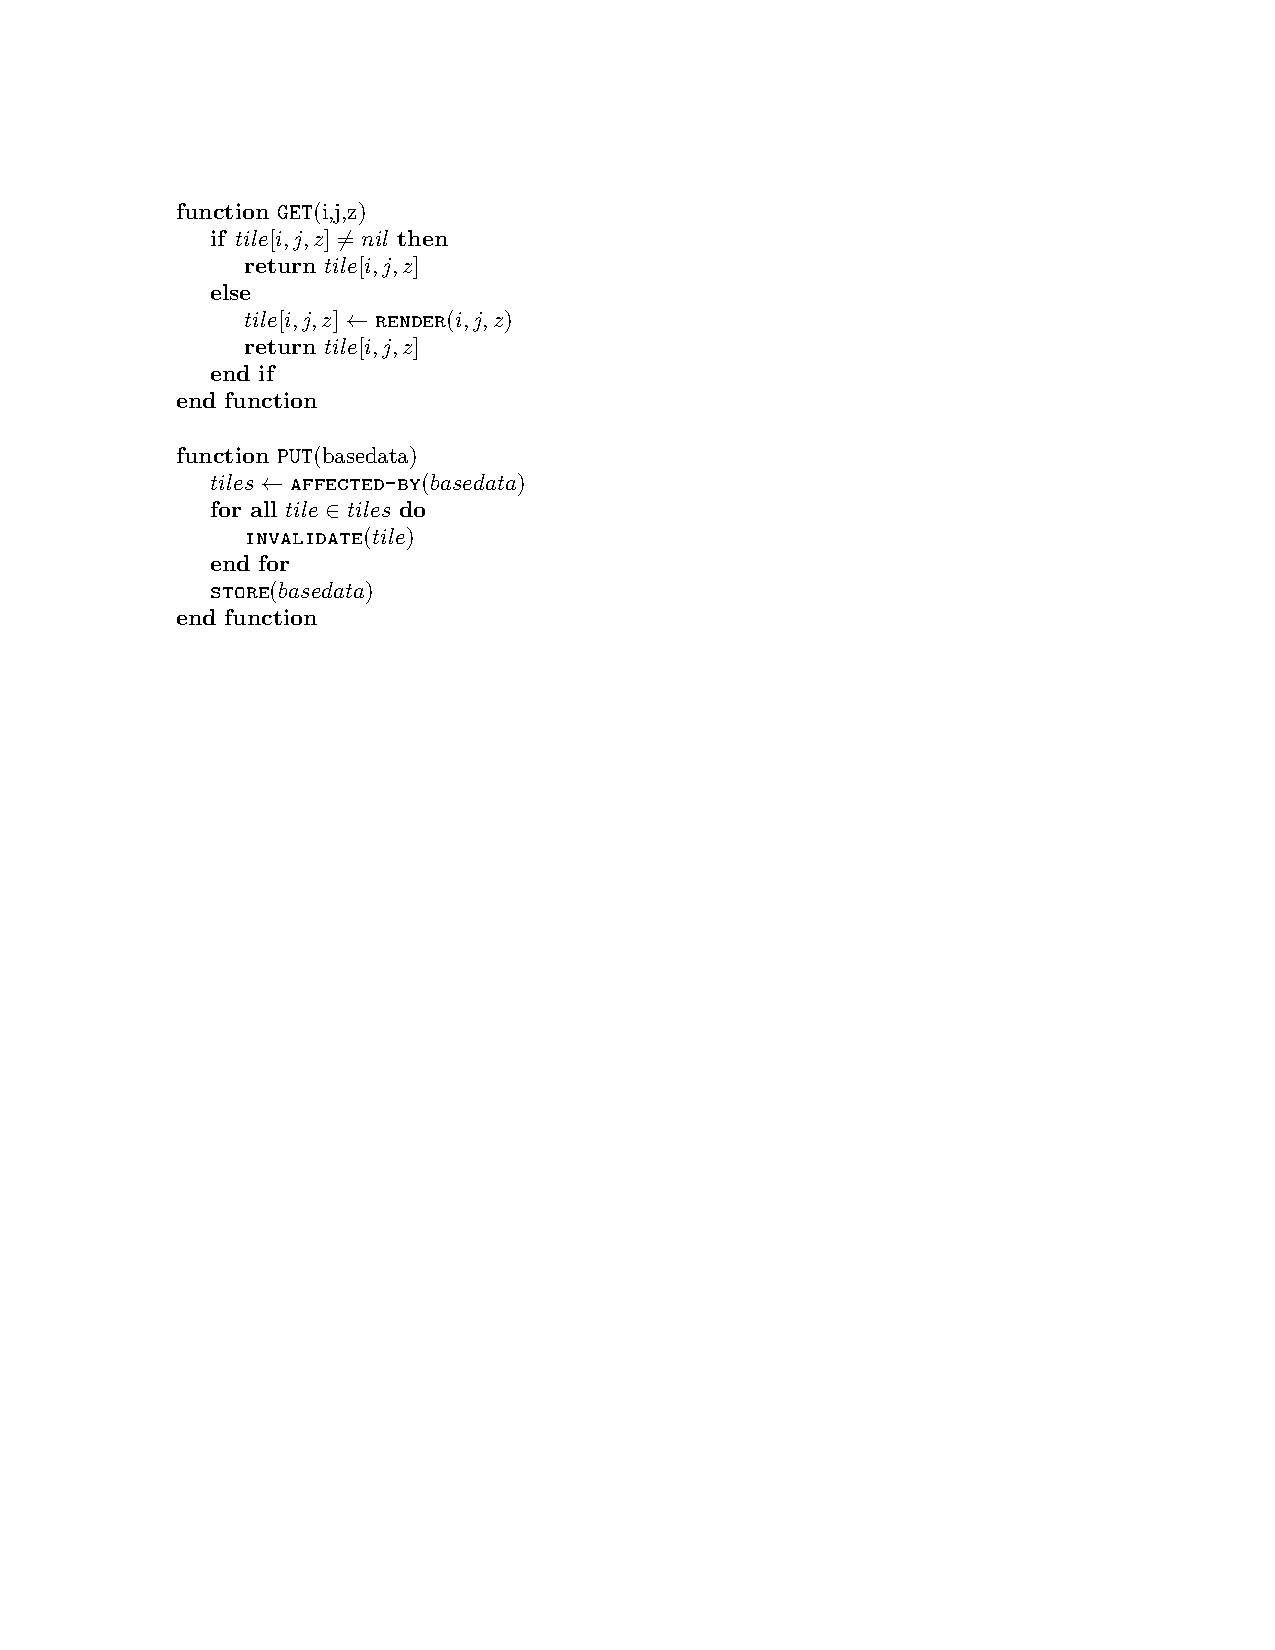
\includegraphics[scale=0.9]{figs-tileheat/pseudocode}
\caption{Processing a \texttt{GET} request: If the tile is materialized, it is returned. Otherwise it is rendered, stored and returned. Processing a \texttt{PUT} request: When base data is updated, the set of tiles that is affected by the change needs to be invalidated.}
\label{fig:pseudocode}
\end{figure}

An invariant maintained by the above functions is that stale tiles are never returned to the user. However, one implementation difficulty typically encountered in practice is that the method for determining the set of tiles that are affected by an update to the base data is not entirely accurate, i.e., a conservative estimate is used in function \texttt{AFFECTED-BY}. This means that sometimes tiles are unnecessarily discarded.

A bounding box request, such as a WMS request, can easily be modeled as a set of \texttt{GET} requests by computing the set of tiles that are intersected inside the \emph{nearest} grid of the tile pyramid. By nearest, we mean the grid that contains tiles with a resolution that best matches the resolution of the bounding box request. Note that these multiple \texttt{GET} requests must be processed against a consistent snapshot. 
%Description of the appropriate implementation details are however beyond the scope of this paper. 

\subsection{The Heatmap model}
\label{sec:heatmap:model}
Given a set of \texttt{GET} requests, we can generate a heatmap of the requests \cite{fisher07}. A heatmap quantifies the number of requests $h_{i,j,z}^t$ that a tile with index $(i,j,z)$ has received in time period $t$. We consider multi-scale heatmaps, which are associated with a tile pyramid. In this work, we only use heatmaps to measure the number of \texttt{GET} requests per tile, but other request types could also be tracked with heatmaps. For example, we could generate heatmaps of \texttt{INVALIDATE} requests, but this is outside the scope of our work.

\subsection{Existing Methods}
\label{sec:existing:methods}
This section covers existing methods for computing and storing a set of tiles for a tile cache.

\minisec{Parallel processing}
Clearly, we need techniques to speed the computation of a tile cache up, given that the number of tiles in a tile pyramid is huge. Using a parallel programming model such as MapReduce \cite{dean04} could reduce computation time of a tile cache by a large factor, but it would require a significant number of machines. In other words, parallelism improves time-to-solution, but does not reduce the amount of resources necessary for the computation. For organizations such as KMS, this high resource cost renders the use of brute-force parallelism unfeasible. A solution is called for to reduce the number of tiles that needs to be computed --- which could then be orthogonally combined with parallelism if available.

\minisec{Detecting duplicates}
A method that reduces storage requirements is to exploit that many tiles are identical, e.g., blue ocean tiles~\cite{mbtile12}. Unfortunately, this solution does not necessarily reduce computation time, given that tiles often must be computed in order to check that they are duplicates. Heuristics have been suggested to predict these duplicated tiles without full computation, but it is unfortunately not easy to decide with absolute certainty~\cite{mbtile12}. We do not know of any published methods that accurately and efficiently predict whether two tiles are the same in the general case without actually computing them, because arbitrary rendering functions are employed.

\minisec{Tile Caching based on Geometries}
A number of authors have suggested methods for predicting the popularity of tiles. Quinn and Gahegan~\cite{quinn10} suggest using certain classes of base objects, like roads and coastlines, as predictors of where people will look at a map. Tiles that are at most 3 miles away from the selected predictors are cached. Conceptually, this approach is based on a model of rational user behavior with fixed rules, and historical workloads are used only to validate the model.

\minisec{GEOM}
KMS currently uses a simplified version of the approach above, which we term \emph{GEOM}. A set of polygons that roughly cover the land areas of Denmark are used to identify the areas that should be fully materialized at all levels of the tile pyramid (levels 1 to 12). Areas outside of these polygons are only materialized at the top-most levels of the tile pyramid (levels 1 to 6)~\cite{lindegaard12}. The resulting partial cache is manageable in size, as roughly $10\%$ of the tile pyramid is materialized. However, the computation time is reported to be between $1.5$ and $2$ days. Tiles are generated by going row-by-row down the levels of the tile pyramid. This is significantly better than random selection, as the highly popular tiles near the top of the pyramid are generated early.

\section{Analysis}
\label{sec:analysis}

In this section, we analyze the request log of a production geospatial web service within KMS, and observe a number of interesting patterns.
The service we examine is the most popular web service of the The Digital Map Supply, a WMS that receives around 800,000 requests per day, and delivers a general purpose background map of Denmark. We report on both temporal (Section~\ref{sec:temporal:characteristics}) and spatial (Section~\ref{sec:spatial:characteristics}) characteristics of the workload.

\subsection{Temporal characteristics of workload}
\label{sec:temporal:characteristics}

\begin{figure}
\centering
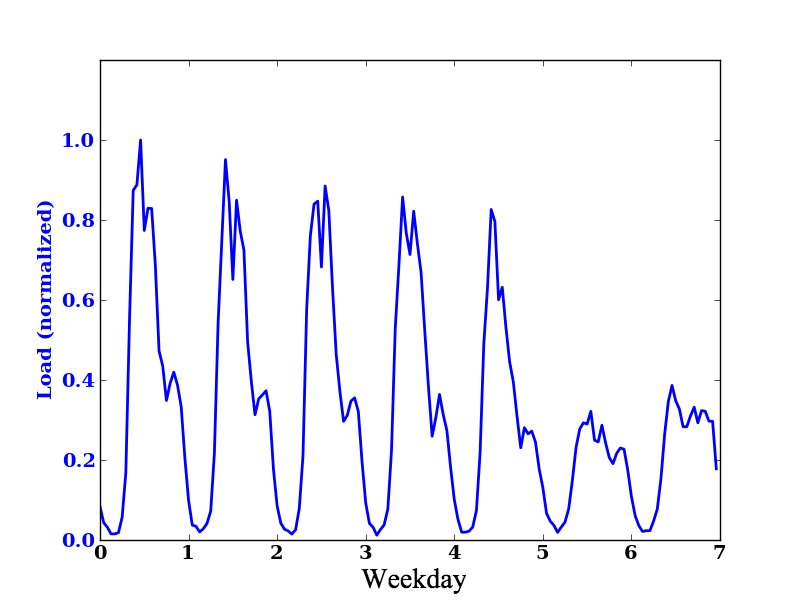
\includegraphics[scale=0.4]{figs-tileheat/average_load_week.png}
\caption{Average load per hour for each day of the week.}
\label{fig:weekload}
\end{figure}

Using a random sample of 90,000 WMS requests from the log, we analyze the workload over time. We have found the following when examining requests processed per second:

\begin{itemize}
\item The load is consistently higher during the middle part of the day, than during other parts of the day.
\item The 24-hour load curves for any two weekdays are very similar.
\item The 24-hour load curves for Saturdays and Sundays are very similar.
\item In general, the load is much higher during weekdays, compared to weekends.
\end{itemize}

These patterns are shown in Figure~\ref{fig:weekload}, where we display the average 24-hour load curve for each day of the week. The curve is generated as an average of all weeks in the log.

\begin{figure}
\centering
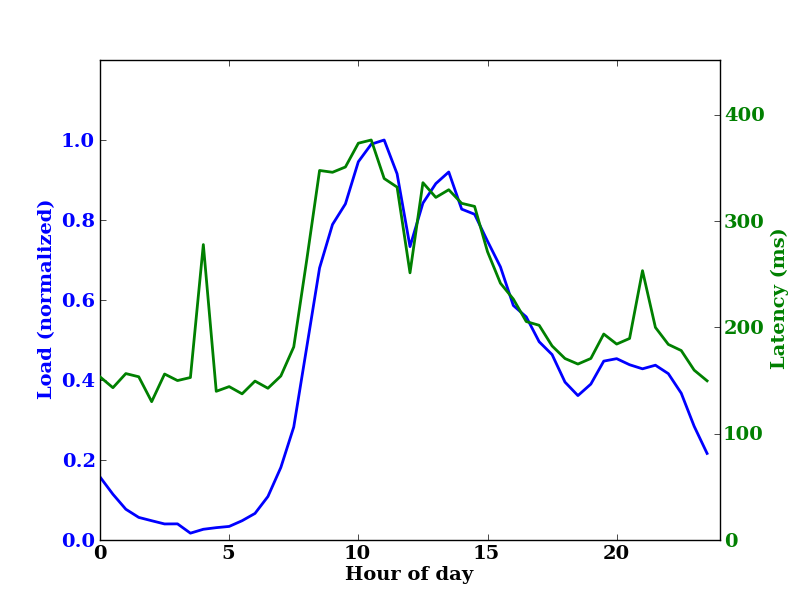
\includegraphics[scale=0.4]{figs-tileheat/correlation.png}
\caption{The correlation between average load (blue) and average latency (green) for 24-hour period.}
\label{fig:correlation}
\end{figure}

We have also looked at the effect of load on latency. In Figure~\ref{fig:correlation}, we plot, side-by-side, the average load and latency curves for a 24-hour period. We observe the following:

\begin{itemize}
\item Load and latency are highly correlated, especially during the periods of high load.
\item The latency effectively doubles when the load is high.
\item Given that weekdays have higher load than weekends, the degradation of latency is most severe in the middle of the day, on weekdays.
\end{itemize}

Our hypothesis is that the increase in latency is caused by increased concurrency and queueing in the system. We have also tested the stability of the load pattern over time by plotting the load for each day over a longer period within the last quarter of 2011. The load patterns can be seen in Figure~\ref{fig:anomaly}. We observe that in general the load curve is very consistent from one weekday to the next, and one week to the next, but anomalies do occur. During week 49 of the last quarter of 2011, the number of requests suddenly doubles. While it is not easy to know what caused such a load spike, it is interesting to ask whether the spike affects the spatial distribution of requests. We examine this question in Section~\ref{sec:spatial:characteristics}.

\begin{figure}
\centering
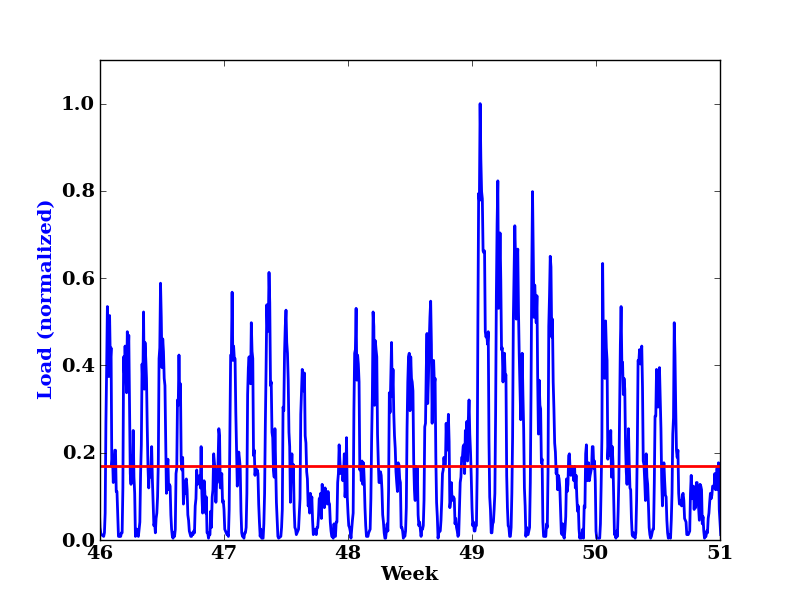
\includegraphics[scale=0.4]{figs-tileheat/anomaly.png}
\caption{Generally stable load, with an anomaly in week 49. The load almost doubles on the first day of week 49. The red line is the average load.}
\label{fig:anomaly}
\end{figure}

\subsection{Spatial characteristics of workload}
\label{sec:spatial:characteristics}
Using heatmaps we have investigated the spatial distribution of requests. We have selected a large number of weekdays, and extracted a full log for these days. The number of log records is significant, with more than 800,000 requests received per day. In Figure \ref{fig:heatmaps}, we show heatmaps for four of these days. We observe that the spatial distribution of requests is quite similar across days. We observe a similar pattern on other days from the log that we have examined.

Given the anomaly in requests per second that we noted in Figure~\ref{fig:anomaly}, we wanted to investigate if the spatial distribution of requests was different for days of increased load compared to normal days. The lower right part of Figure~\ref{fig:heatmaps} shows a heatmap for the day with unusually high load. The spatial distribution is slightly different compared to the other three heatmaps, but still very similar. The data indicates that the spatial distribution of requests is similar for weekdays, and largely independent of fluctuations in load. Using the notation we defined for heatmaps this means that

\[
h_{i,j,z}^t \approx h_{i,j,z}^{t+1}
\]

\begin{figure}
\centering
\begin{tabular}{|c|c|}
\hline
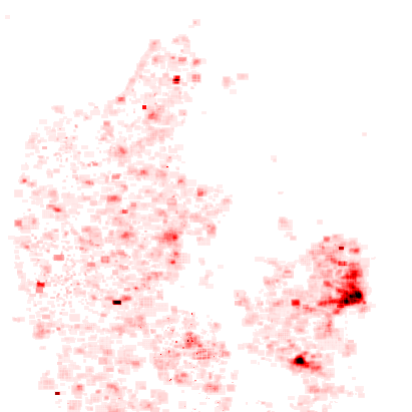
\includegraphics[scale=0.22]{figs-tileheat/heatmap-e_1.png} & 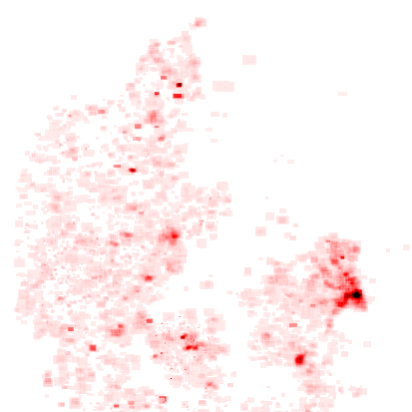
\includegraphics[scale=0.22]{figs-tileheat/heatmap-e_2.png} \\
\hline
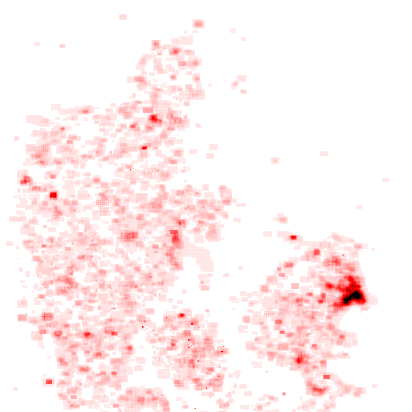
\includegraphics[scale=0.22]{figs-tileheat/heatmap-e_3.png} & 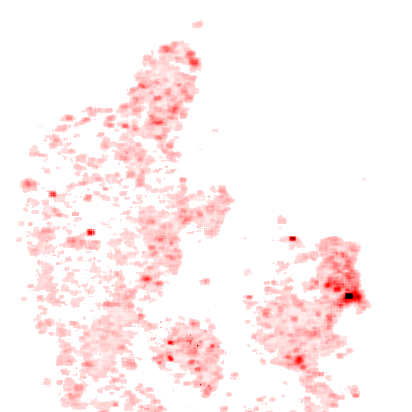
\includegraphics[scale=0.22]{figs-tileheat/heatmap-e_4.png} \\
\hline
\end{tabular}
\caption{Heatmap of spatial distribution of requests for four consecutive days (resolution $\mathbf{3.2}$ meter/pixel). The spatial distribution is similar but not equal. The day in the lower right corner is the day with very high load identified in Figure \ref{fig:anomaly}.}
\label{fig:heatmaps}
\end{figure}

%In Figure~\ref{fig:skew}, we show the cumulative distribution function of tile access frequencies, which has been computed from the heatmaps. 
We observe that the frequency of tile access is highly skewed; other studies have concluded the same, namely that the spatial distribution of \texttt{GET} requests follows a power law \cite{fisher07,talagala00}. We also observe that the skew increases with resolution, i.e., with  levels of the tile pyramid that contain more tiles. 

In general, this means that the set of tiles needed for a tile cache with a high hit ratio is smaller than one might expect. The main goal of our work and the algorithms we have developed is to explore how small such a cache can be, while still delivering high hit ratios on user requests.

\section{TileHeat framework}
\label{sec:algorithms}

In this section, we present the TileHeat framework for selecting and caching tiles. We begin with an overview of the framework and the context it is used in (Sections~\ref{sec:tileheat:overview} and~\ref{sec:tileheat:tasks}), followed by two different algorithms for tile ranking (Sections~\ref{sec:heat:hw} and~\ref{sec:heat:d}).   

\vspace{4ex}

\subsection{Overview}
\label{sec:tileheat:overview}
Based on our observations of the workload in Section \ref{sec:analysis}, we have designed the TileHeat framework for a repeated cycle of time periods containing a high- and low-load window. This basic cycle is outlined in Figure~\ref{fig:high:low}.

The life cycle of a system that uses TileHeat to manage tiles is as follows: We organize processing in TileHeat into a sequence of \emph{time periods}. Each time period is composed of two \emph{time windows}: the high-load window and the low-load window. Throughout both windows, the geospatial web service is available for clients and therefore must carry out normal processing of user requests, i.e., \texttt{GET} and \texttt{PUT}. During the low load window, however, we can additionally \emph{select and pre-compute tiles} that we expect to be accessed during the next time window, based on access patterns observed for previous time periods. In the following, we describe how we carry out the selection and pre-computation of tiles.

\begin{figure}
\centering
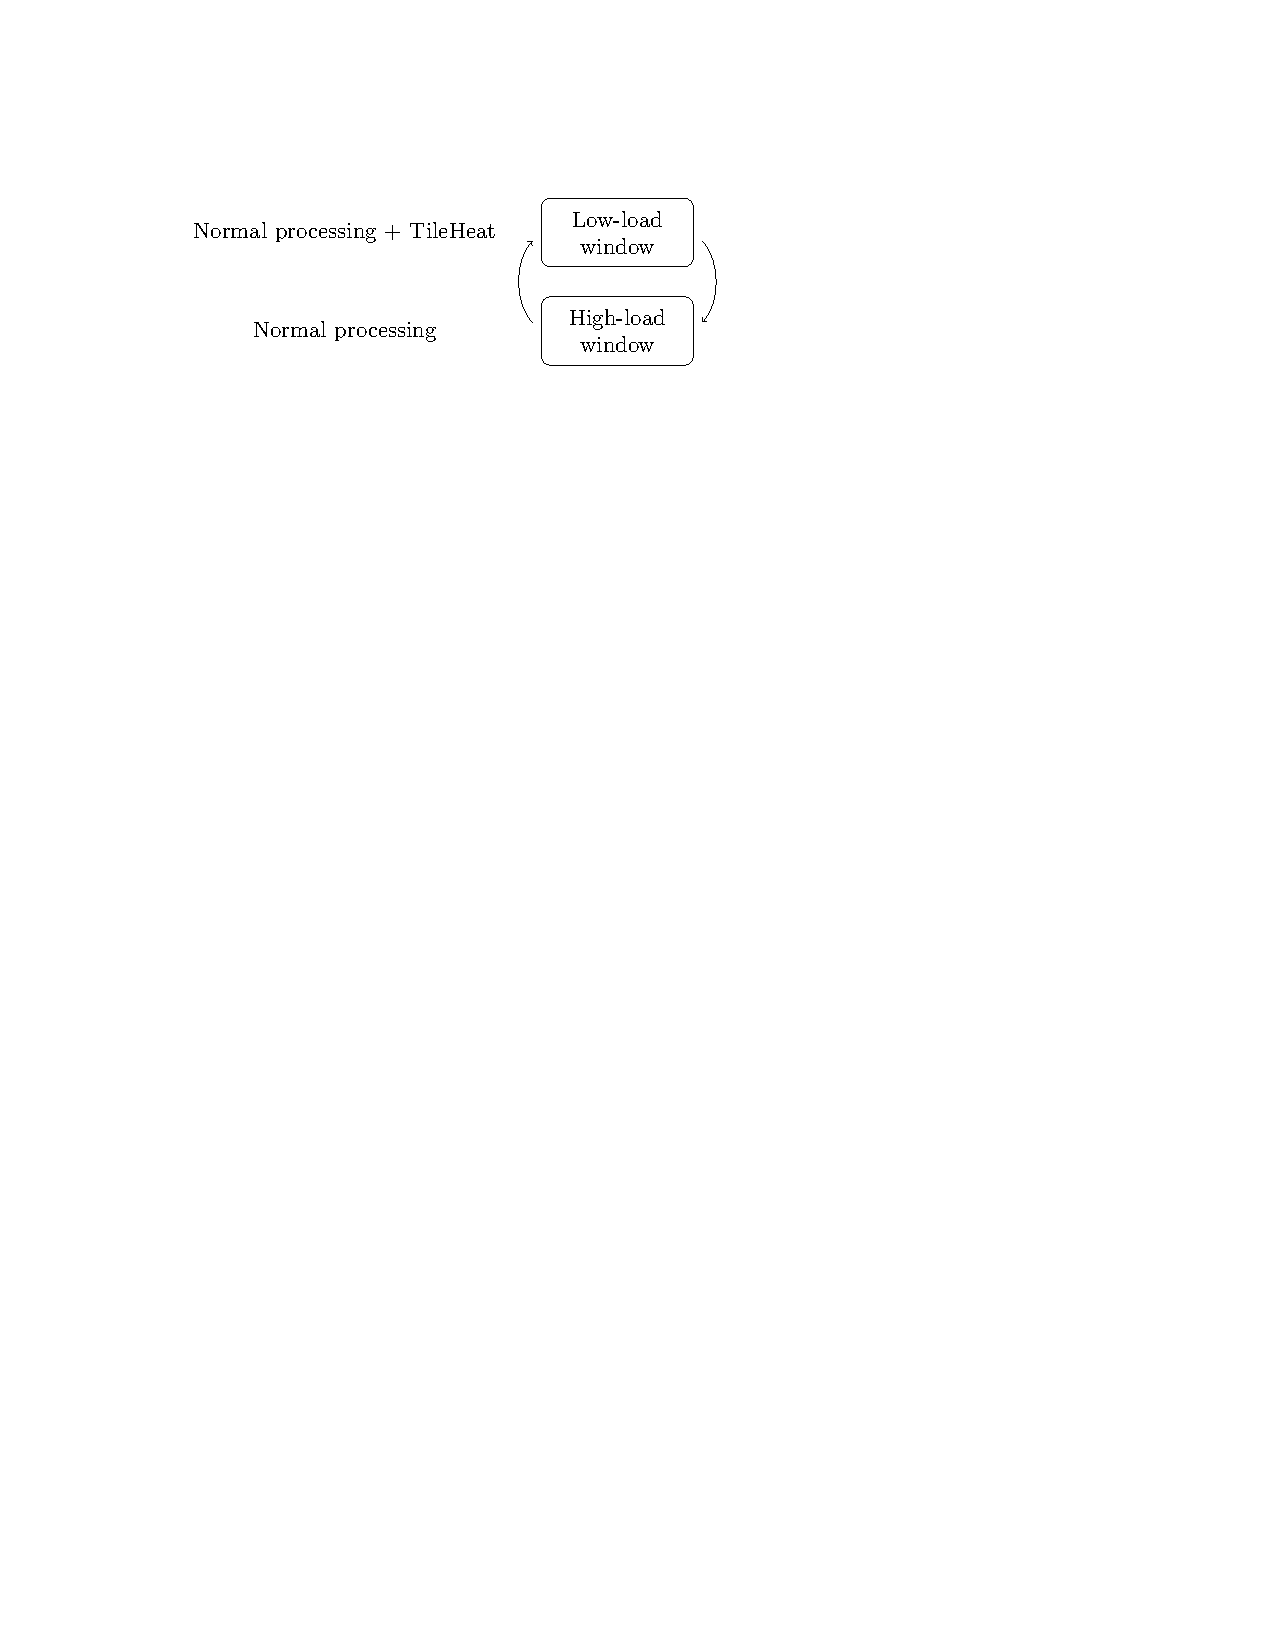
\includegraphics[scale=0.8]{figs-tileheat/figoverview}
\caption{Time periods and time windows: Processing during high- and low-load windows.}
\label{fig:high:low}
\end{figure}

%We assume that the base data from which the tiles are generated, gets updated frequently, which makes it a bad strategy to compute the entire set of tiles. 

\subsection{Tasks performed by TileHeat}
\label{sec:tileheat:tasks}

TileHeat is a framework for embedding tile selection algorithms into a log analysis procedure. The log analysis procedure computes a set of $n$ heatmaps, and passes these to tile selection. Tile selection in turn employs a \emph{prediction algorithm}, which predicts the heatmap for time $t + 1$. TileHeat uses the predicted heatmap to select which tiles to materialize for the next high-load window. 

The following steps are performed in time period $t+1$ by the TileHeat framework:
%
\begin{enumerate}
\item A prediction algorithm uses heatmaps for time periods $t-n$ to $t$ to predict the heatmap for time period $t+1$.
\item The tiles in the predicted heatmap are sorted in non-increasing order by heat.
\item The $k$ first tiles that are not already materialized are selected.
\item The materialization of the $k$ tiles is scheduled.
\end{enumerate}

The number $k$ is chosen as the number of tiles that can be materialized during the current low-load window. Various algorithms can be used to predict the heatmap for $t + 1$. In this work, we present two algorithms for the TileHeat framework: HEAT-HW (Section~\ref{sec:heat:hw}) and HEAT-D (Section~\ref{sec:heat:d}).

The running time of TileHeat can be estimated as follows. Let $m$ be the number of requests in the request log for time periods $t-n$ to $t$. We assume that the number of \texttt{GET} requests for each log request is bounded by a constant. The number of tile requests is therefore $O(m)$. By using a hash table, we can build the heatmaps in (expected) $O(m)$ time. As the sorting step takes at most $O(m)$ tiles as input, the (expected) running time of TileHeat is $O(m \log m)$ --- plus the running time of the prediction algorithm. 

\subsection{HEAT-HW algorithm}
\label{sec:heat:hw}
We have developed the HEAT-HW algorithm, which uses exponential smoothing applied to the heatmaps for time periods $t-n$ to $t$. Specifically, we use Holt-Winter double exponential smoothing~\cite{chatfield88}, which takes the trend of the observed variable into account. We motivate our choice of smoothing function in two ways:

\begin{enumerate}
\item We apply a smoothing function in general to avoid overfitting to the training data. Although the data we have analyzed is very stable, we introduce smoothing to prepare the algorithm for less stable workloads.
\item We use Holt-Winter smoothing in particular because it captures the trend in popularity for each tile. In future work, we would like to make use of the trend to adapt proactively to sudden rises in popularity for a geographical subregion by increasing the number of nodes serving those tiles. This of course implies a multi-node cache.
\end{enumerate}

Exponential smoothing is applied by treating each heat tile index $(i,j,z)$ as a separate variable. The equations for double exponential smoothing for heatmaps are given below (assuming that the first time period is $0$).

\begin{eqnarray*}
s_{i,j,z}^0 & = & h_{i,j,z}^0 \\
b_{i,j,z}^0 & = & h_{i,j,z}^1 - h_{i,j,z}^0 \\
s_{i,j,z}^{t+1} & = & \alpha h_{i,j,z}^0 + (1 - \alpha)(s_{i,j,z}^{t} + b_{i,j,z}^{t} ) \\
b_{i,j,z}^{t+1} & = & \beta (s_{i,j,z}^{t+1} - s_{i,j,z}^{t}) + (1 - \beta) b_{i,j,z}^{t}  \\
\end{eqnarray*}

As defined in Section~\ref{sec:heatmap:model}, $h_{i,j,z}^t$ is the observed heat of tile $(i,j,z)$ in time period $t$; $s_{i,j,z}^t$ is the smoothed value for time $t$ and $b_{i,j,z}^t$ is the trend for time $t$. Parameters $\alpha$ and $\beta$ are determined experimentally.

\subsection{HEAT-D algorithm}
\label{sec:heat:d}
The exponential smoothing as used in HEAT-HW only ranks tiles that are actually requested in the training data. Often, the training data is sparse, or tiles that are not accessed in the time periods $t-n$ to $t$ get accessed in time $t+1$, due to local changes in the spatial distribution of tile requests. 

HEAT-D is inspired by Tobler's first law of geography: ``Everything is related to everything else, but near things are more related than distant things''. HEAT-D works by applying a dissipation step to all heatmaps prior to applying Holt-Winter double exponential smoothing. The dissipation step is similar to the Jacobi method used for numerically solving the heat equation~\cite{templates}.

The following steps are performed by HEAT-D: 

\begin{enumerate}

\item For each heatmap of time periods $t-n$ to $t$, apply $p$ iterations of the dissipation step. An iteration consists of moving a fraction of the heat of each cell $(i,j,z)$ to its eight neighbors. This fraction is controlled by  a dissipation constant $\mu$. The corresponding differences in heat applied to each cell are shown in Figure~\ref{fig:dissipate}. 

\item Apply HEAT-HW over the heatmaps obtained in the step above. 

\end{enumerate}

%We apply $p$ rounds of the dissipation step to each heatmap in the training data. For each index $(i,j,z)$ in the heatmap, the dissipation step moves a fraction of the heat for that tile to its eight neighbors, based on a dissipation constant $\mu$. The process is illustrated in Figure~\ref{fig:dissipate}.

\begin{figure}
\centering
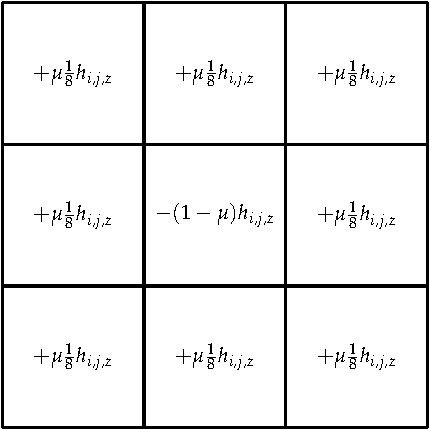
\includegraphics[scale=1]{figs-tileheat/disspate2}
\caption{Each dissipation step transfers heat from a center cell to each of it's eight neighbors. The center cell $(i,j,z)$ loses $(1 - \mu) h_{i,j,z}$ heat, and the neighbors gain $\mu \frac{1}{8} h_(i,j,z)$ heat. This is repeated for all center cells that are not on the border of the heatmap, using double buffering to avoid prematurely updating the heat of a cell.}
\label{fig:dissipate}
\end{figure}

The result of running dissipation on a sparse sample set can be seen in Figure~\ref{fig:dissipate_before_after}.

\begin{figure*}
\centering
\begin{tabular}{ll}
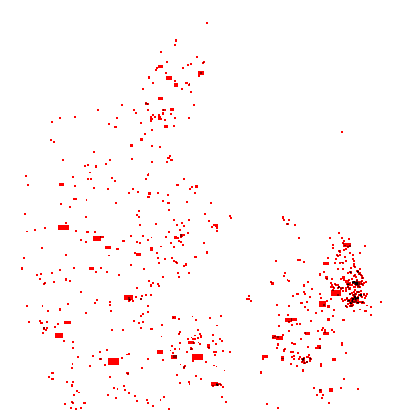
\includegraphics[scale=0.5]{figs-tileheat/heat_d-before.png} & 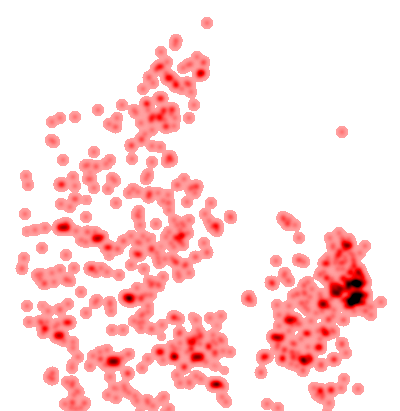
\includegraphics[scale=0.5]{figs-tileheat/heat_d-after.png} \\
\end{tabular}
\caption{Result of running the dissipation algorithm on a sparse heatmap (left) which contains $1.25\%$ of the samples used to create the heatmaps of Figure~\ref{fig:heatmaps}. The result (right) covers the hot regions of the heatmaps in Figure~\ref{fig:heatmaps} much better.}
\label{fig:dissipate_before_after}
\end{figure*}

\section{Experiments}
\label{sec:experiments}

The goal of our experiments is to show the improvements that can be gained by TileHeat in real production workloads. We first describe our experimental setup (Section~\ref{sec:setup}) and then present results (Section~\ref{sec:results}).  
%in a real production setting. We use real production workloads to test the hit ratio of the selected tile sets. 

\subsection{Experimental setup}
\label{sec:setup}

Here we describe how we have executed the experimental evaluation of our algorithms using a production request log extracted from KMS. Due to constraints in both time and access to the production system, we have not actually materialized the tiles selected by our methods, so we could not measure the effect this would have on latency in a production environment. Assuming, however, that serving tiles from cache is much more CPU- and I/O-efficient than computing on demand, we believe that the effect would be significant, given the high hit ratios we are able to achieve (Section~\ref{sec:results}). 

\subsubsection{Datasets}
\label{sec:datasets}
To validate the algorithms we have developed, we have extracted six datasets from the KMS request log for the last quarter of 2011. The method we used was to randomly select six weekdays, and for each of these days, select the $n$ previous weekdays to be used as training data. We use $n=3$. 

%Each dataset thus consists of the following:
%
%\begin{itemize}
%\item One weekday to use for validation.
%\item Three previous weekdays to use as training data. 
%\end{itemize}

The size of the log of requests for each weekday is substantial, with over 800,000 WMS requests per day, which we translate into \texttt{GET} requests. 

\subsubsection{Methodology}
\label{sec:methods}

This section describes our experimental methodology. The algorithms we have tested are:

\begin{itemize}

\item OPT: the optimal algorithm, which builds a heatmap of the workload used for the validation, and uses this heatmap to select the tiles. 

\item GEOM: the method currently employed by KMS, described in Section~\ref{sec:existing:methods}.

\item HEAT-HW: our heatmap method with Holt-Winter double exponential smoothing, described in Section~\ref{sec:heat:hw}. For HEAT-HW, the best set of parameters we could devise was $\alpha = 0.2$ and $\beta = 0.1$. 

\item HEAT-D: our heatmap method extended with dissipation, described in Section~\ref{sec:heat:d}. For HEAT-D, we set $\mu = 0.05$. The number of iterations $p$ is calibrated according to the resolution of the heatmap being dissipated. Given a scale factor $s$, we set $p = s \times (\text{\#rows}+\text{\#columns})/2$. The intuition is that heatmaps with higher resolution need more iterations of the dissipation step in order to cover enough geographical area. We set $s = 0.002$. 

\end{itemize}

The methodology we have developed to test the algorithms consists of playing back the production request log, both to train the algorithms, and to validate their performance. The outline of the method is as follows:

\begin{enumerate}
\item Pick a random day $t$.
\item Compute $n$ heatmaps for the $n$ consecutive days leading up to and including $t$.
\item Compute the actual heatmap for day $t+1$ from the data. 
\item Normalize the cells of the actual heatmap for day $t+1$ by the sum of heat for all cells. Now, each cell in the actual heatmap contains the fraction of the hit ratio contributed by the corresponding tile for day $t+1$. 
\item Calculate the tile ranking for the OPT algorithm by sorting tiles according to normalized heat contained in the actual heatmap.
\item For each of the other algorithms, obtain the corresponding tile ranking for day $t+1$, and measure the hit ratio by cumulating normalized heat from the actual heatmap.    
%\item The $n$ heatmaps are given as input to the algorithms GEOM, HEAT-HW, HEAT-D, and the output consists of the corresponding predictions of the heatmap for day $t+1$.
%\item Independently sort the cells of the two predicted heatmaps by decreasing heat, obtaining two lists of sorted cells.
%\item For each list, iterate over the cells, starting with the cell with highest heat. For each cell, look up the heat of the corresponding cell in the actual heatmap for day $t+1$, and plot these heat values cumulatively.
\end{enumerate}


Our results show averages of the hit ratios obtained by running the algorithms against each of the six datasets, recalling that a dataset consists of three days used to train the algorithms, and one day used to validate the performance of the algorithm.

\subsection{Results}
\label{sec:results}

\begin{figure*}
\centering
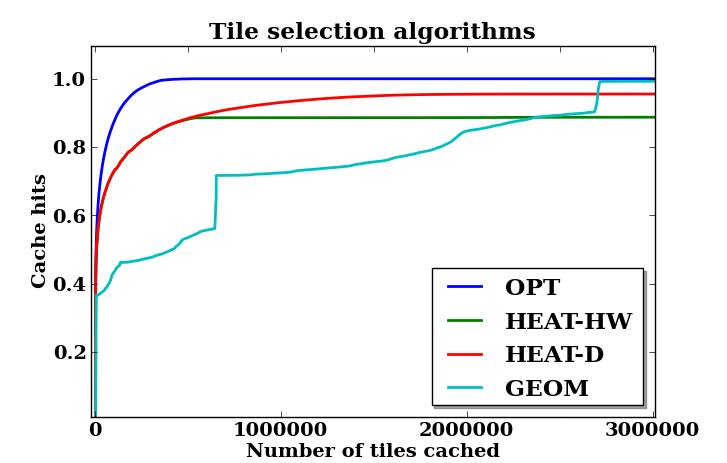
\includegraphics[scale=0.4]{figs-tileheat/results_closeup2.png}
\caption{The performance of tile selection algorithms for the first 3 million tiles selected, using three days of training data. The result is averaged over several runs using different data sets.}
\label{fig:results}
\end{figure*}

In Figure \ref{fig:results}, we show the average hit ratios obtained by the algorithms we have developed for TileHeat, using the datasets described in Section \ref{sec:datasets}. 
The figure shows the hit ratio of the first three million tiles that are selected by the algorithms. A full materialization contains more than ten million tiles. OPT, however, has a $100\%$ hit ratio after selecting 500,000 tiles. 

%OPT has a $100\%$ hit ratio after selecting 500,000 tiles.  %We also compare our algorithms against GEOM, which is the tile selection algorithm currently used by KMS.
As mentioned previously, the throughput of materializing tiles has been measured by KMS to be $58$ tiles per second on their infrastructure. A time window of $7.2$ hours fits inside the low load time period from $10$ PM to $6$ AM. During this window, we can compute $1.5$ million tiles. Within this tile budget, our best algorithm, HEAT-D, achieves a hit ratio of $95\%$. GEOM achieves a hit ratio of $76\%$ within the same tile budget. The hit ratio of HEAT-D is thus $25\%$ better than GEOM for this tile budget.

In general, we see that our algorithms rise significantly faster towards high hit ratios for small sets of tiles, e.g., in the 500,000 tile range. It is also clear that HEAT-D outperforms HEAT-HW after 500,000 tiles, and overall dominates HEAT-HW. This is because HEAT-D ranks more tiles than HEAT-HW, i.e., by ranking tiles that are not requested in the training workloads. We conclude that the additional tiles boost the hit ratio significantly, which confirms our hypothesis that tiles that are near to each other have similar access frequencies.

At around $2.6$ million tiles, GEOM overtakes HEAT-D, and becomes optimal. A peculiar effect of GEOM is a staircase effect that can be seen in Figure~\ref{fig:results}. We believe that this is an artifact of the way GEOM selects tiles --- selecting row-by-row the tiles that intersect the geometries provided. At certain latitudes, the rows cross over highly popular areas like the capital of Denmark, Copenhagen. The city of Copenhagen is clearly visible as a high-heat, dark area in the right side of each of the heatmaps shown in Figure~\ref{fig:heatmaps}. There are several steps in the staircase, as this effect is repeated at higher resolutions.

\section{Related work}
\label{sec:related}

Caching of dynamic web content has been extensively studied in a number of contexts~\cite{DDT+01:DynamicContentAcceleration,GMA+08:Ferdinand,GLR05:GoodEnough,LGZ04:MTCache,LKM+02:DBCache,Moh01:WebCaching}. A major issue investigated by these proposals is the policy used to keep the cache up-to-date. 
For example, Guo et al.~\cite{GLR05:GoodEnough} propose a set of declarative constraints that specify presence,  consistency, completeness, and currency of cached content. 
Garrod et al.~\cite{GMA+08:Ferdinand} explore how to take advantage of multiple cache servers while maintaining consistency. In contrast, our workload analysis shows that the main challenge for a geographical web service is the computational expense of the refresh procedure of the tile cache, rather than the freshness of relatively slowly updated map data. In this sense, our approach can be seen as similar to periodically refreshing a materialized view. This  ``view'' delivers the tile pyramid based on the underlying geographical data; however, it is both spatial and includes external user-defined functions to compute tile content. While similar in spirit to the materialized-view approach of MTCache~\cite{LGZ04:MTCache}, the additional complexities of our domain render the problem harder in several ways: First, not all of the view definition is available to the system, making it more difficult to predict which tiles are affected by which data and recompute selectively. Second, only portions of the view are of interest to end users, due to skew in access patterns, and it is not obvious how to define which portions are interesting ahead of time. Third, computation of tiles is a very resource-intensive user-defined function, making even a partial refresh of the spatial cache costly.  
 
Our work can also be seen as a self-tuning approach to managing a tile web cache~\cite{CN07:SelfTuning10YrPaper}. Similarly to online self-tuning approaches, such as COLT~\cite{SAMP07:COLT} and the seminal COMFORT~\cite{WHMZ94:COMFORT} project, TileHeat operates on a feedback loop, collecting workload characteristics, performing reasoning for choosing a new system configuration, and introducing configuration changes as necessary. However, our work differs in both the characterization of the problem as well as in the design choices we make for each step of our feedback loop. 
In particular, our choices are motivated by a careful analysis of the production log of a country-wide geographical web service. 
%We derive several conclusions from the analysis: 1) The access patterns of the rendering service exhibit high regularity, with low activity off day hours; 2) Access patterns can be largely inferred based on historical data, 3) The cost for materialization of tiles for caching is significant, and consequently services with moderate update rates -- such as geographical web services -- can dramatically profit from a selective cache.  

Adaptive algorithms have been studied for the classic buffer cache replacement problem, including 2Q~\cite{JS94:2Q}, ARC~\cite{MM03:ARC}, and LRU-K~\cite{OOW93:LRU-K}. Our work, however, is focused on the different scenario of spatial web caching, in which tiles are materialized in advance of processing the workload.
% Unlike previous caching algorithms, our approach takes advantage of the capability to observe the workload for a given time period, and uses the collected data to materialize a spatial cache for the next period.  
As in semantic caching~\cite{DFJ+96:SemanticCaching}, we exploit application characteristics to decide what data to cache and update. In contrast to semantic caching, we exploit spatial properties for higher web cache hit ratios, such as with our heat dissipation method. 
	
The basic idea of using heat to measure popularity of data items arises naturally in applications with skewed access patterns. For example, Scheuermann et al.~\cite{SWZ93:DiskCooling} propose schemes for data placement and adaptive load balancing that "cool" disks by redistributing file fragments. In spatial services more specifically, many researchers have observed that there is a strong skew in the access frequencies of tiles, and that this skew follows a power law~\cite{fisher07,LGXF12:SpatialPrefetching,talagala00}. Li et al.~\cite{LGXF12:SpatialPrefetching} exploit skew to create a pre-fetching model of spatial tiles, with focus on predicting short-term user navigation. Their work is based on a substantial body of related short-term prediction approaches~\cite{KKK01:Prefetching,KKK01:Prefetching2,LKK+02:Prefetching}. These methods are optimized for pre-fetching  tiles seconds before they are requested by a user. The amount of pre-fetching done during a time period is thus proportional to the load. As we have observed, load and latency are proportional, which means that pre-fetching in real time does little to alleviate load peaks. To reduce the high latency caused by load peaks, we instead pre-compute tiles during periods of low load. To achieve this, we develop methods that do not rely on the input of individual users browsing a map in real time. 
%In contrast, we look at the problem of pre-computing a large set of tiles that comprise a production-grade spatial web cache. 

As discussed in Section~\ref{sec:existing:methods}, Quinn and Gahegan~\cite{quinn10} suggest using certain classes of base objects, such as roads and coastlines, as predictors of where users will look at a map. However, as observed in Fisher's study of Microsoft Hotmap~\cite{fisher07}, real-world workloads can contradict models of rational user behavior, exclusively focused on a fixed set of rules. An example given by Fisher~\cite{fisher07} was a banner ad that caused frequent requests for ``empty'' parts of the Pacific Ocean. Based on such observations of real-life events, Fisher develops a multi-scale descriptive model that quantifies web map usage based on a heatmap. Their study supports our observation that anomalous patterns may be transient in time, but partially detectable from a training data set. In contrast to Fisher, however, we exploit this insight to propose multiple strategies to keep hit ratios on a spatial web cache high, while at the same time drastically reducing resource consumption during recomputation of tiles. 

\section{Conclusion}
% What we did
In this work, we propose and evaluate the use of heatmaps to analyze the request log for a geospatial service as well as to improve the creation time of a tile cache for this service. 
As we have observed, heatmaps can be made predictive and aid in selecting a set of high traffic tiles. We applied our techniques to the request log of a production system and showed that substantial improvements over an existing method were attained. In particular, using our HEAT-D algorithm to compute a tile cache yields a $25\%$ improvement in the hit ratio for a reasonable time window of materialization. HEAT-D accurately predicts the popularity of tiles that are not requested in the training data by employing a heat diffusion process. 

% Future work
While our results improve on existing methods, for future work we plan to do a more thorough exploration of the parameter space of the algorithms HEAT-HW and HEAT-D to investigate if further improvements could be achieved. In addition, we plan to work on efficient methods for materializing the tiles selected by our algorithms as well as use the trend information from HEAT-HW to build a distributed cache that adapts to sudden spikes in load. 
%Exploring efficient methods of materializing the tiles, given a plan computed by TileHeat, would bring the work full circle. 
Finally, deploying TileHeat in a production environment and measuring the effect on latency remains as an important direction of future work.
